\documentclass[tikz]{standalone} % border={left bottom right top}
\usepackage{tikz}
\usepackage{tikz-3dplot}
\usetikzlibrary{shadings,decorations.markings,arrows.meta,quotes,angles,snakes,decorations}
\usepackage{xcolor}
\usepackage{amsmath}
\usepackage{marvosym}

\tikzset{
    %Define standard arrow tip
    >=stealth'
}

\tikzset{
    tst/.style={
      thin, opacity=0.5,
      dashed
    },
    my-arc/.style={
      start angle=0, end angle=360,radius=0.4
    }
}

\tikzset{
    ->-/.style={
        decoration={markings, mark=at position #1 with {\arrow{>}}},
        postaction={decorate}
    },
    scatter/.style={decorate, draw=black,
        decoration={complete sines,amplitude=8pt, segment length=11pt}}
}

\definecolor{blue}{RGB}{92, 96,176}
\definecolor{red}{RGB}{223, 99,140}
\definecolor{green}{RGB}{83,192,97}
\definecolor{yellow}{RGB}{253,216,112}
\definecolor{gray}{RGB}{109,109,109}
\definecolor{lightgray}{RGB}{200,200,200}
\definecolor{orange}{RGB}{239,142,79}

% \newcommand{\bbox}[1]{%
%   \color{red!50}\rlap{\fbox{$\phantom{#1}$}}%
%   \color{black}#1%
% }

\def\cTens#1#2#3 {
    \begin{scope}[shift={#3}]
        	\fill[#1] (0,0) circle (#2);
        	\clip (0,0) circle (#2);
	\shade[outer color=#1, inner color=#1!70] (-#2,#2) circle (1.75*#2);
	\draw[very thin] (0,0) circle (#2);
		\end{scope}
}

\def\rTens#1#2#3#4 {
	\begin{scope}[shift={#4}]
	        	\fill[#1] (-#2/2,-#3/2) rectangle (#2/2,#3/2);
	        	\clip (-#2/2,-#3/2) rectangle (#2/2,#3/2);
		\shade[outer color=#1, inner color=#1!70] (-1.41*#2/2,1.41*#3/2)  circle (1.3*#3/2+1.3*#2/2);
		\draw[very thin] (-#2/2,-#3/2) rectangle (#2/2,#3/2);
	\end{scope}
}

\def\oTens#1#2#3 {
    \begin{scope}[shift={#3}]
        	\fill[#1] (0,0) circle (#2);
        	\clip (0,0) circle (#2);
	\shade[outer color=#1, inner color=#1!70] (-#2,#2) circle (1.75*#2);
	\draw[very thin] (0,0) circle (#2);
		\end{scope}
}

%!TEX root = thesis.tex
%%%%%%%%%%%%%%%%%%%%%
\def\ri{\mathrm i}
\def\re{\mathrm e}
\def\rd{\mathrm d}
\def\rD{\mathcal D}
\def\hc{{\rm h.c.}}
\def\tr{{\rm tr}}
\def\C{\mathcal{C}}
\def\DC{\Delta\C}
\def\GX{\Gamma X}
\def\DCav{\overline{\Delta\C}}
\def\up{\uparrow}
\def\down{\downarrow}
\def\pdag{{\vphantom\dag}}
\def\pp{\vphantom{n'}}
\def\Cav{\overline\C}
\def\MH{H}
\def\HS{\mathcal{H}}
\def\FS{\mathcal{F}}
\def\omegaT{\tilde{\omega}}
\def\tbc{{\\[1cm]\bf \color{red}[TO BE CONTINUED...]}}
\newcommand{\ave}[1]{\langle #1 \rangle}
\newcommand{\sign}[1]{\text{sign}\left( #1 \right)}
\newcommand{\commutator}[1]{\left[ #1 \right]}
\newcommand{\anticommutator}[1]{\left\{ #1 \right\}}
\newcommand{\brlr}[1]{\left( #1 \right)}
\newcommand{\abs}[1]{\left| #1 \right|}

\usepackage{braket}
\begin{document}

\tikzset{
    %Define standard arrow tip
    >=stealth'
}

\tikzset{
    tst/.style={
      thin, opacity=0.5,
      dashed
    },
    my-arc/.style={
      start angle=0, end angle=360,radius=0.4
    }
  }

\tikzset{
    tst/.style={
      thin, opacity=0.5,
      dashed
    },
    my-arc2/.style={
      start angle=0, end angle=360,radius=0.2
    }
  }

\definecolor{blue}{rgb}{0.2745098039, 0.5333333333, 0.9450980392}
\definecolor{red}{rgb}{0.9176470588, 0.2588235294, 0.2078431373}
\definecolor{yellos}{rgb}{0.9764705882, 0.7333333333, 0.1764705882}
\definecolor{green}{rgb}{0.2039215686, 0.662745098, 0.3176470588}


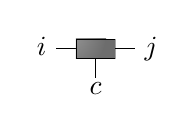
\begin{tikzpicture}
    \node (rw1) at (0,0) {};
    \draw ($(rw1)+(-0.5,0)$) node[left] {$i\vphantom{j}$} --($(rw1)+(.5,0)$) node[right] {$j\vphantom{i}$};
    \coordinate (1) at ($(rw1)+(-0.5,-.125)$);
    \foreach \y in {1}{
        \draw ($(1)+(0.5,0)$) coordinate (1) -- ++(0,-0.25);
    }
    \node[below,yshift=-.175cm] at (1) {$c$};
    \rTens{gray}{.5}{0.25}{(rw1)}
\end{tikzpicture}


\end{document}
